\documentclass{a0poster}

\usepackage{fancytikzposter} 
\usepackage{booktabs}
\usepackage{marvosym}

%%%%% --------- Change here if you want ---------- %%%%%
%% margin for the geometry package, must be changed before using the geometry package
%% default value is 4cm
 \setmargin{2.5}

%% the space between the blocks
%% default value is 2cm
\setblockspacing{0.6}

\usetemplate{2}


%%% size of the document and the margins
%% A0
% \usepackage[margin=\margin cm, paperwidth=118.9cm, paperheight=84.1cm]{geometry} 
\usepackage[margin=\margin cm, paperwidth=84.1cm, paperheight=118.9cm]{geometry}
%% B1
% \usepackage[margin=\margin cm, paperwidth=70cm, paperheight=100cm]{geometry}



%% changing the fonts
\usepackage{cmbright}
%\usepackage[default]{cantarell}
%\usepackage{avant}
%\usepackage[math]{iwona}
\usepackage[math]{kurier}
\usepackage[T1]{fontenc}


%% add your packages here
%\usepackage{hyperref}  % % DISABILITATO I VIRTUAL REF


% % % DAN ADDED
\newtheorem{thm3}{Proposition}

% % % END DAN ADDED

\title{Sequence-based Recommendation with Bidirectional LSTM Network} %Networking-Computing resource allocation for Hard Real-Time Green Cloud applications}
%\author{Elena Botoeva\\
%  KRDB Research Centre, Free University of Bozen-Bolzano, Italy\\
%  \texttt{botoeva@inf.unibz.it}
%}
\author{Hailin Fu , Jianguo Li , Jiemin Chen , Yong Tang , Jia Zhu\\ %\vspace{20pt}
	hailin@m.scnu.eud.cn - 510000, \\
	 \textbf{School of Computer Science, South China Normal University} 
	 % 19-23 June '16 - Trento (Italy)
   }

\begin{document}

%%%%% ---------- the background picture ---------- %%%%%
%% to change it modify the macro \BackgroundPicture
\ClearShipoutPicture
\AddToShipoutPicture{\BackgroundPicture}

\noindent % to have the picture right in the center
\begin{tikzpicture}
  \initializesizeandshifts
  % \setxshift{15}
  % \setyshift{2}


  %% the title block, #1 - shift, the default value is (0,0), #2 - width, #3 - scale
  %% the alias of the title block is `title', so we can refer to its boundaries later
  \ifthenelse{\equal{\template}{1}}{ 
    \titleblock{47}{1}
  }{
    \titleblock{47}{1.5}
  }

  %% a logo can be added to the title block
  %% #1 - anchor relative to the title block, #2 - shift, #3 - width, #3 - file name
   \ifthenelse{\equal{\template}{2}}{ 
     %\addlogo[south west]{(2,0)}{6cm}{unibz_b.png}
     \addlogo[south west]{(-5,0)}{12cm}{logos/SCNU.png} 
     \addlogo[south west]{(63,0)}{12cm}{logos/SCNU.png}
   }{
     \addlogo[south west]{(0,0.2)}{11cm}{logos/SCNU.png} 
     \addlogo[south west]{(48,0.2)}{11cm}{logos/SCNU.png}
   }


  %% a block node, with the specified position (optional), title and the content
  %% #1 - where (optional), #2 - title, #3 - text
  %%%%%%%%%% ------------------------------------------ %%%%%%%%%%
  \blocknode{Abstract}
  {%\emph{
  	\vspace{-10pt}
    In modern recommendation systems, most methods often neglect the sequential relationship between items. So we propose a novel Sequence-based Recommendation model with Bidirectional  Long Short-Term Memory neural network (\Large BiLSTM4Rec \normalsize ) which can capture the sequential feature of items to predict what a user will choose next. By collecting consumed items of a user in a sequence with time ascending order, fitting the model with the last item as the label, the rest items as the features, we regard this recommendation assignment as a super multiple classification task. Once trained well, the output layer of our model will export the probabilities of the next items with given sequence. In the experiments, we compare our approach with several commonly used recommendation methods on a real-world dataset. Experimental results indicate that our sequence-based recommender can perform well for short-term interest prediction on a sparse, large dataset.
  }
  
  \vspace{80pt}
  \blocknode%
  {Introduction}%
  { 
  	The primary assignments of recommendation systems faced with consist of two parts: ratings predicting and products recommendation. So to predict what a user will choose next given his consumed history is one of the crucial mission \cite{Wan2015NextBR} in recommendation area. In many websites and applications, such as online electronic business, news/videos website, music/radio station, they need an excellent service for users to recommend what they will like in future. Existing recommenders mainly concentrate on finding the neighbor sets for users or items, or leveraging other explicit/implicit information (such as tags, reviews, item contents and user profiles) for neighborhood-aware. However, to the best of our knowledge, few works use the sequential feature of data to build recommender. We find that the sequence of data implicates much exciting and relevant information, for example in a video website, the user who watched "Winter is coming" (S01, E02 of Game of Thrones) will be more likely to watch "The Kingsroad" (S01, E02 of Game of Thrones). Even at the 2011 Recsys conference, Pandora's researchers gave a speech about music recommendation and said they found many users consumed music in sequences.

    Our work was inspired by the previous study of Siwei Lai et al. \cite{AAAI159745}, where a neural network is proposed to capture the sequence of words in a sentence.  We took a similar approach by considering one item as a word, the catalog of items as a vocabulary, and the historical consumed items of one user as a sentence, to capture the sequence of the user consumed items.

  }
  
  
   %%%%%%%%%% ------------------------------------------ %%%%%%%%%%
   %\blocknodew[($(currenty)-(3.5,0)$)]{30}{Variable Width Block Nodes} %
   \blocknode %
   {Architecture} %
   {
   Let us assume that $\mathbb{U}= \left \{ u_{1},u_{2},...,u_{N} \right \}\label{eq}$ is the user set and $\mathbb{I}= \left \{ i_{1},i_{2},...,i_{M} \right \}$ is the item set. For each user $u$, there is an observed consumed items sequence $\mathbb{S}_{u}=\left \{ s_{u}^{1},s_{u}^{2},...,s_{u}^{t-1},s_{u}^{t} \right \}$ in ascending order of time, where $s_{u}^{t}$ is the item consumed by user $u$ at time $t$. The sequential prediction problem is to predict $s_{u}^{t+1}$ for each user $u$.

    \vspace{-20pt}  	
      	\begin{tikzfigure}[Framework of sequence-based recommendation]
      	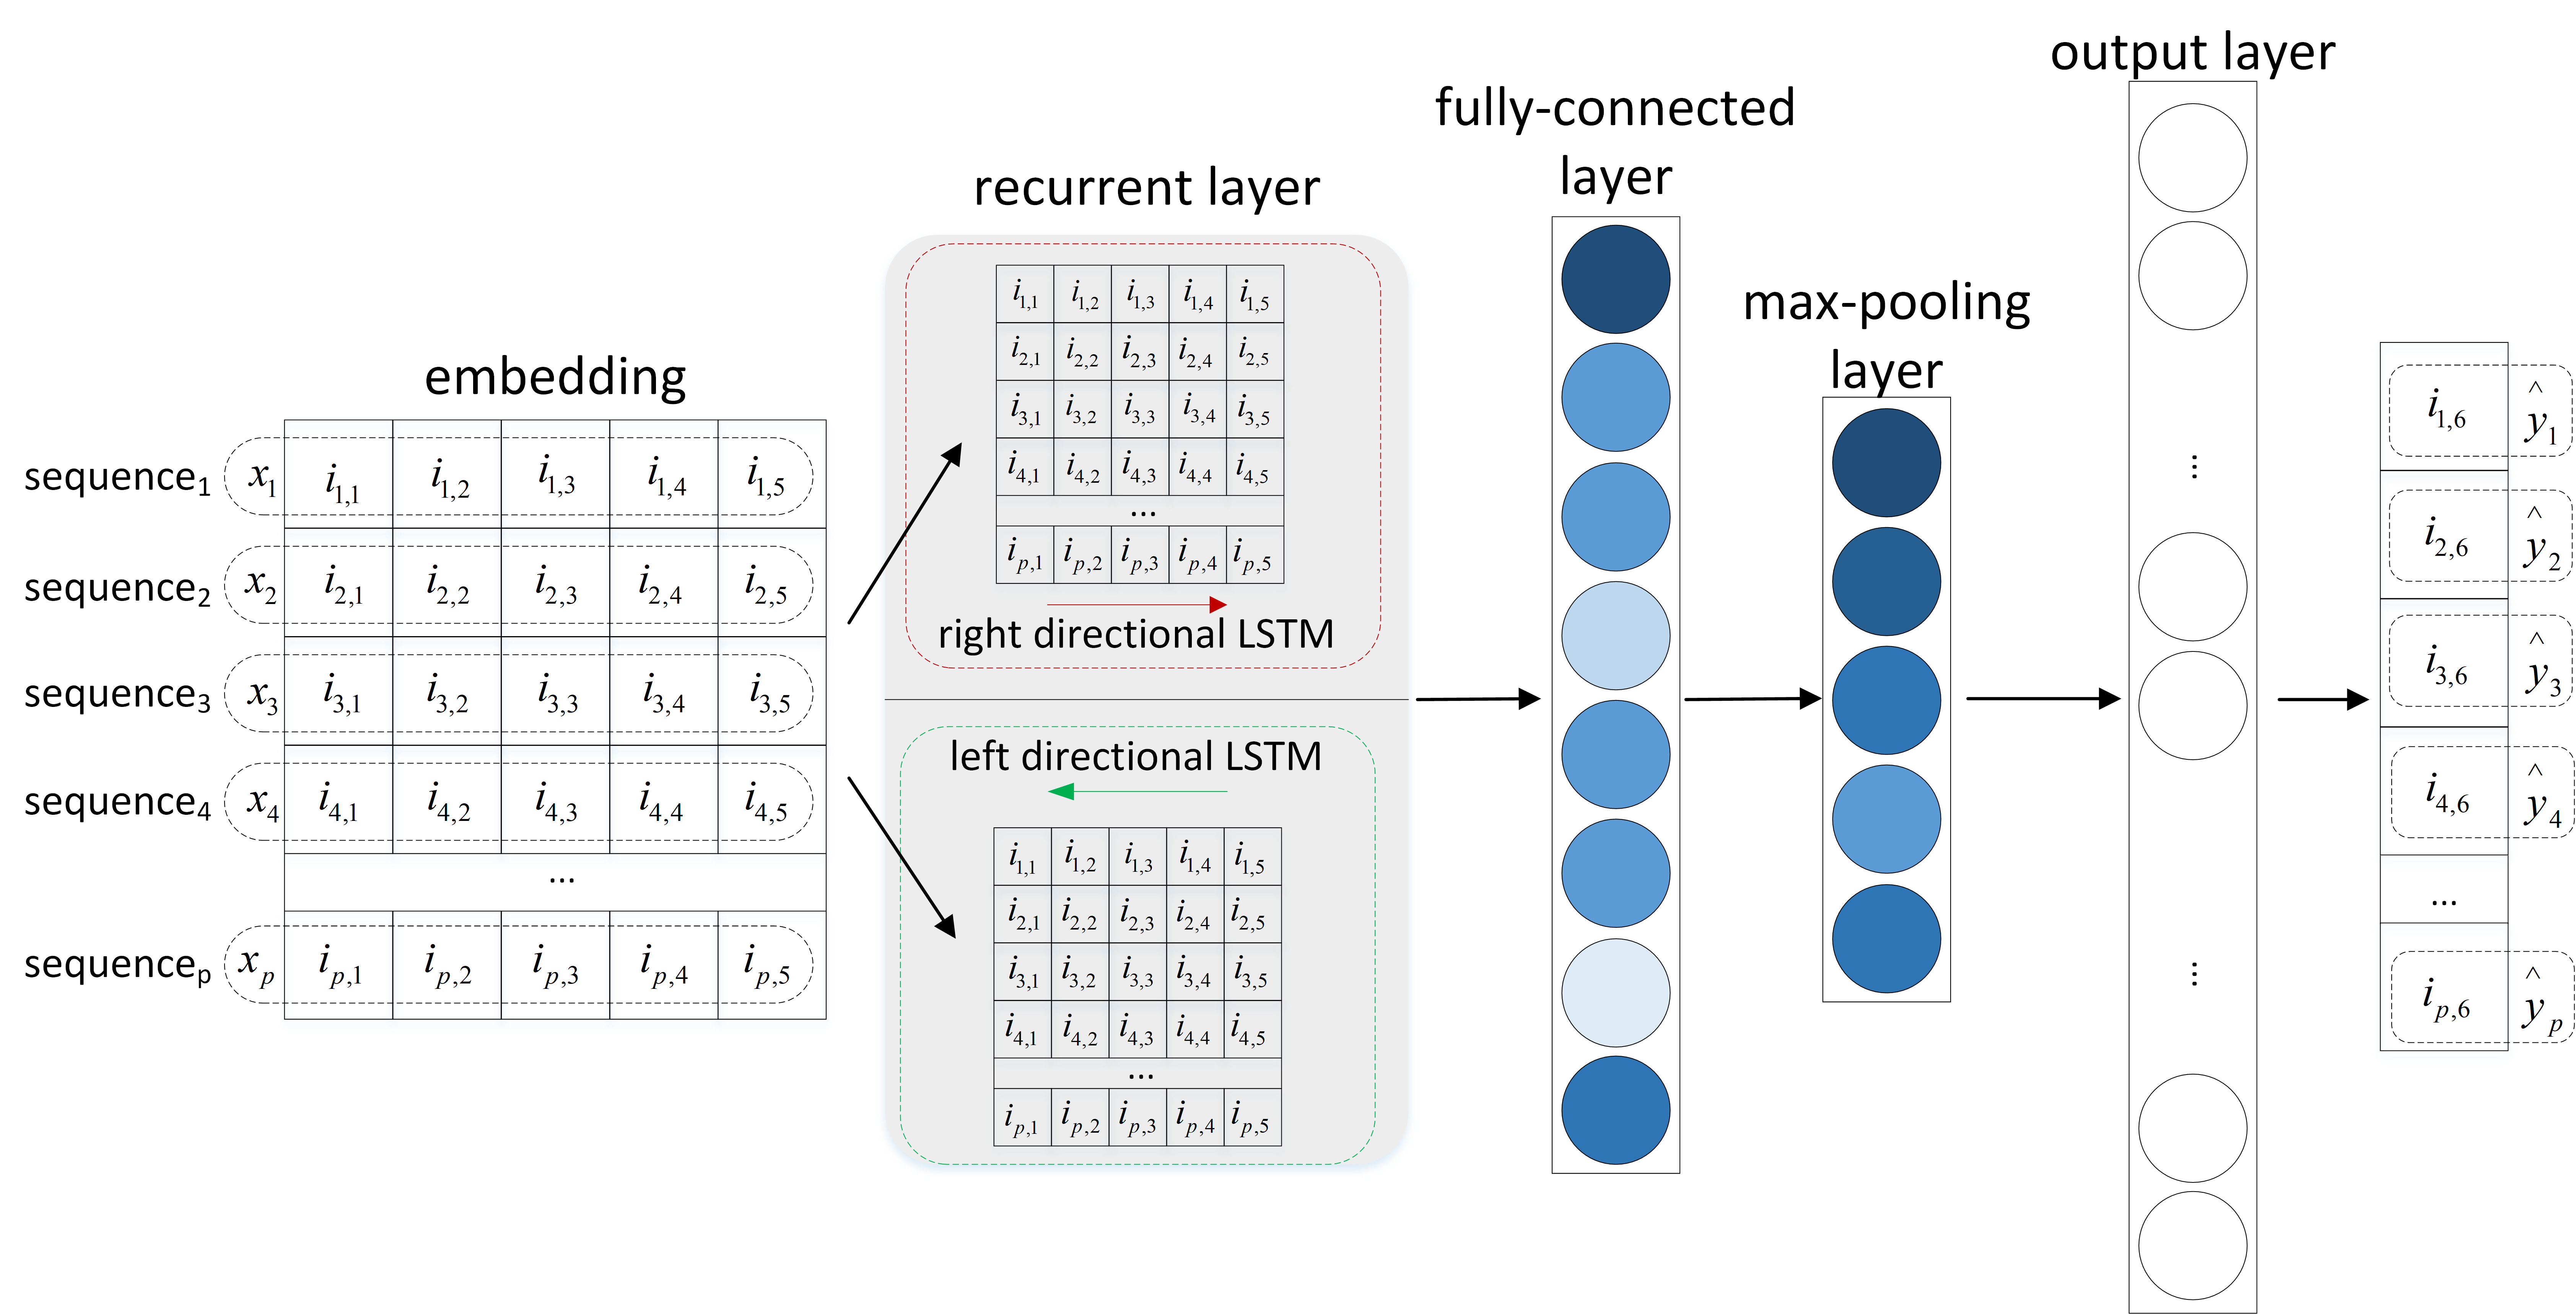
\includegraphics[width=1 \columnwidth]{images/structer.png}
      	\end{tikzfigure}

      We propose a novel deep neural model to capture the sequence feature of the user's consumed data. Our model mainly consists of five layers: embedding, recurrent structure, fully-connected layer, pooling layer and output layers. Figure 1 shows the structure of our sequence-based recommender.
   }
   
     \blocknode %
  {} %
  {
  \bibliographystyle{plain} % Plain referencing style
  \bibliography{sample} % Use the example bibliography file sample.bib
  }

  \blocknode %
  {Get contacted!} %
  {

  \begin{minipage}{0.8\textwidth}
        %\begin{figure}%            <!-- new
        BiLSTM4Rec is currently hosted on GitHub and I am working as a recommendation algorithm engineer intern at \textit{CloudBrain.ai}. Experience exchanging, academic discussion and contributions are strongly encouraged! \\[0.5em]
      \huge \Mundus \normalsize \hspace{0.5cm} \textbf{https://github.com/fuhailin/BiLSTM4Rec}
        %\end{figure}               <!-- new
    \end{minipage}%
    \begin{minipage}{0.2\textwidth}
        %\begin{figure}%
        
\includegraphics[width=0.5\textwidth]{logos/GitHub-Mark.png}%
        %\end{figure}
    \end{minipage}
  }
 	
	\startsecondcolumn


	 %%%%%%%%%% ------------------------------------------ %%%%%%%%%%
	 \blocknode{Mathematical Section}%
	 {
	 	Word Embedding shines in the field of Natural Language Processing, instead of ending up with huge One-hot encoded vectors we also can use an embedding matrix to keep the size of each vector much smaller:
\begin{equation}
e(I_{i})=EI_{i}
\label{eqn:Einstein}
\end{equation}
\begin{eqnarray}
h_{b}(I_{i})=\sigma (W^{(b)}h_{b}(I_{i-1})+W^{(cb)}e(I_{i-1})) \\ 
h_{a}(I_{i})=\sigma (W^{(a)}h_{a}(I_{i+1})+W^{(ca)}e(I_{i+1}))
\end{eqnarray}
\begin{eqnarray}
x_{i}=[h_{b}(I_{i});e(I_{i});h_{a}(I_{i})]
\end{eqnarray} 

\begin{equation}
y_{i}^{(2)}=tanh(W^{(2)}x_{i}+b^{(2)})
\end{equation}
\begin{equation}
y^{(3)}=\max_{i=1}^{n}y_{i}^{(2)}
\end{equation}
\begin{equation}
y^{(4)}=W^{(4)}y^{(3)}+b^{(4)}
\end{equation}
Finally, a softmax activation function applied to $y^{(4)}$, which can convert the output values to the probabilities of next items.
\begin{equation}
p_{i}= \frac{e^{y_{i}^{(4)}}}{\sum_{k=1}^{n}e^{y_{k}^{(4)}}}
\end{equation}

We define all of the parameters to be trained as $\theta $.
\begin{equation}
\theta=  \left \{ E,b^{(2)},b^{(4)},h_{b}(B_{1}),h_{a}(B_{n}),W^{(2)}, W^{(4)},\right.\\
\left.W^{(b)},W^{(a)},W^{(b)},W^{(cb)},W^{(ca)} \right \} \\
\end{equation}
The training target of the network is to minimize the categorical cross entropy loss:

\begin{equation}
\mathcal{L}(y,S,\theta )=-\sum_{u\in \mathbb{U}}[y_{u}\log p(y_{u}|S_{u},\theta)+(1-y_{u})\log (1-p(y_{u}|S_{u},\theta ))]
\end{equation}		
	}


  %%%%%%%%%% ------------------------------------------ %%%%%%%%%%
  %\blocknodew[($(currenty)-(3.5,0)$)]{30}{Variable Width Block Nodes} %
  \blocknode %
  {Results} %
  {
  	
  	\vspace{-30pt}
  		\begin{minipage}[t]{1.0 \linewidth}
  		\flushleft
  		\begin{tikzfigure}[The training results of BiLSTM4Rec model on 80\% LiveStreaming-10M with different Time Windows]

  		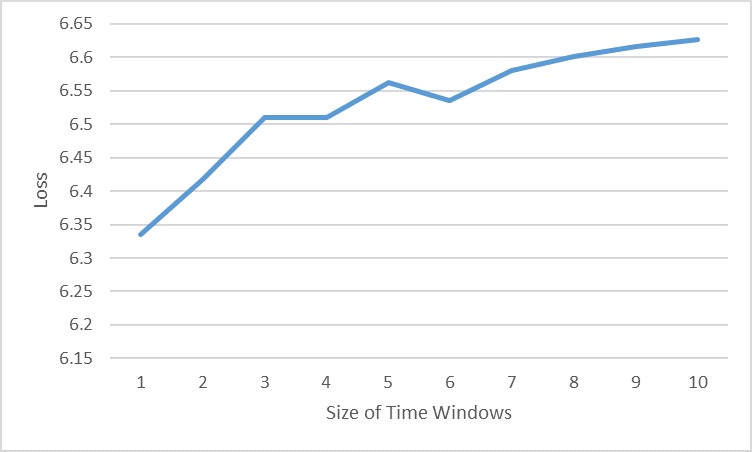
\includegraphics[width=0.45\columnwidth]{images/Loss_timewindows.png} %\\
  		 %\label{fig:3a}
  		% \vspace{10pt}
  		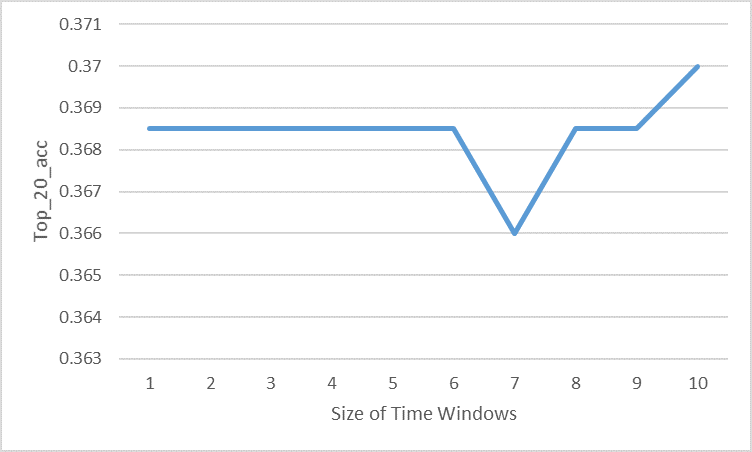
\includegraphics[width=0.45\columnwidth]{images/Top_20_acc_timewindows.png}\label{fig:3}
  		\end{tikzfigure}
  		\end{minipage}

      \begin{minipage}[t]{1.0 \linewidth}
      \flushleft
      \begin{tikzfigure}[BiLSTM4Rec training on 80\% LiveStreaming-10M with Time Windows as 5, and recommends items with the top 20 probability values]

      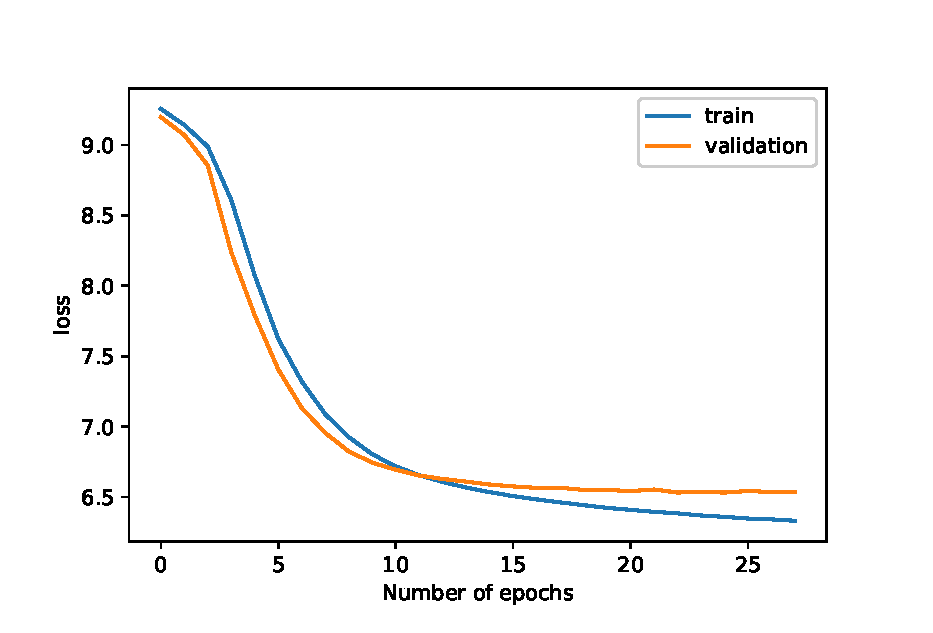
\includegraphics[width=0.45\columnwidth]{images/model_loss} %\\
       %\label{fig:3a}
      % \vspace{10pt}
      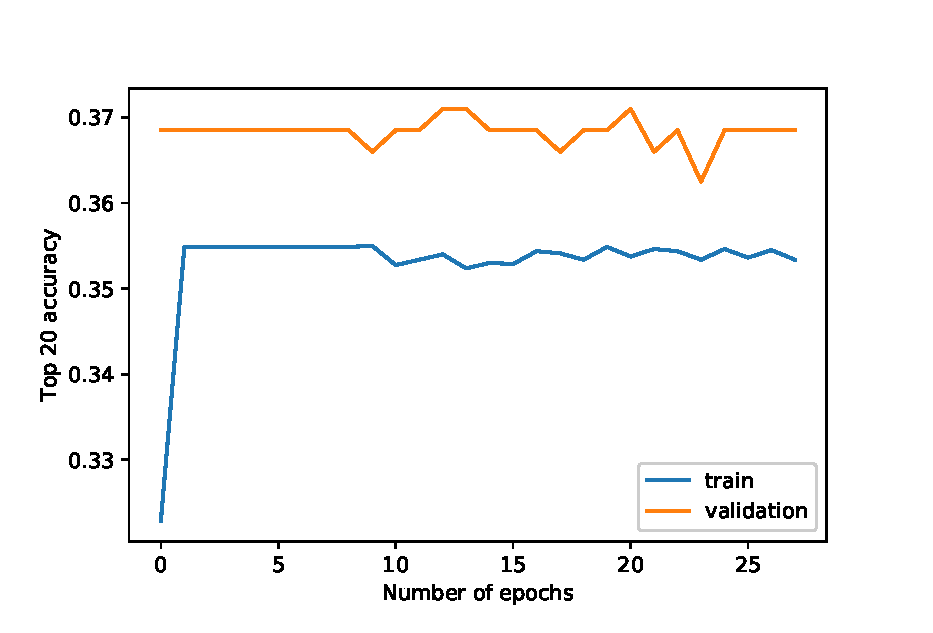
\includegraphics[width=0.45\columnwidth]{images/Top_20_accuracy}\label{fig:3}
      \end{tikzfigure}
      \end{minipage}
	}

     \blocknode %
     {Comparisons} %
     {
\begin{center}\vspace{1cm}
\begin{tabular}{*{6}{l}}
\toprule
\textbf{Metrics}& \textbf{POP}& \textbf{UBCF}& \textbf{IBCF}& \textbf{LSTM}& \textbf{BiLSTM4Rec} \\
\midrule
Precision@1& 0.0056& 0.0108 & 0.0112 & 0.1135 & \textbf{0.1165} \\
\hline
Recall@1& 0.0056& 0.0108 & 0.0112 & 0.1135 & \textbf{0.1165}\\
\hline
F1@1& 0.0056& 0.0108 & 0.0112 & 0.1135 & \textbf{0.1165}\\
\hline
Precision@5& 0.00018& 0.0476 & 0.006223 & 0.0463 & \textbf{0.0488}\\
\hline
Recall@5& 0.0009& 0.0476 & 0.0313 & 0.2315 & \textbf{0.244}\\
\hline
F1@5& 0.0003& 0.0476 & 0.010433333 & 0.077167 & \textbf{0.081333}\\
\hline
Precision@20& 0.00015& \textbf{0.1154} & 0.004705 & 0.01825 & 0.01895\\
\hline
Recall@20& 0.003& 0.1154 & 0.0941 & 0.365 & \textbf{0.379}\\
\hline
F1@20& 0.000285714& \textbf{0.1154} & 0.008961905 & 0.034762 & 0.036095\\
\bottomrule
\end{tabular}
\end{center}\vspace{1cm}
     }
     
  %%%%%%%%%% ------------------------------------------ %%%%%%%%%%
  \plainblock{($(currenty)$)} %-(xshift) + (xshift) -(yshift) %[($(currenty)+(0,10)$)]%
  {38}{Conclusion} %
  {
  	BiLSTM4Rec is a novel recommendation by modeling recent consumed items as a "sentence" to predict what users will choose next. We introduced the Bidirectional Long Short-Term Memory neural network to a new application domain: recommendation system. We dealt with consumed items sequences by embedding matrix to save memory cost, and the final model can learn short-term interest of the user. Experimental results show that our approach outperforms existing methods to a great extent, and shows it is suitable to do a short-term prediction. Moreover, it doesn't have an unacceptable time complexity.
  } 

\end{tikzpicture}


\end{document}




